\documentclass[a4paper, 12pt]{article}
\usepackage{graphicx}
\usepackage{mathtools}
\usepackage{color}
\usepackage{epstopdf}
\usepackage[UTF8]{ctex}
\usepackage{listings} 
\usepackage{xcolor}
\usepackage{courier} % 可选,使用Courier字体,类似Jupyter中的代码字体  
  
\lstset{  
    basicstyle=\ttfamily\small, % 设置基本字体样式和大小  
    keywordstyle=\color{blue}, % 设置关键字样式  
    stringstyle=\color{red}, % 设置字符串样式  
    commentstyle=\color{green}, % 设置注释样式  
    breakatwhitespace=false, % 不在空白处自动换行  
    breaklines=true, % 允许自动换行  
    captionpos=b, % 将标题放在底部  
    frame=single, % 为代码块添加单线框(可选)  
    numbers=left, % 在左侧显示行号  
    numberstyle=\tiny\color{gray}, % 设置行号样式  
    tabsize=4, % 设置制表符宽度为4个空格  
    showstringspaces=false % 不在字符串中显示空格标记      
}  
\begin{document}
    {\huge\title{实验报告}}
    {\large\author{程传哲}}
    \date{\today}
    \maketitle
\section{学习成果}

\subsection{调试与性能分析}
\begin{enumerate}
  \item{\large 打印调试}
    \begin{itemize}
        \item 在python中我们可以使用print输出变量查看,得到信息以便调试内容
        \item 同理在c++中可以使用cout或者printf
    \end{itemize}
  \item{\large 日志调试}
    \begin{itemize}
        \item 可以将日志写入文件,也可以根据严重等级过滤日志
    \end{itemize}
    \begin{lstlisting}
$ python logger.py
# Raw output as with just prints
$ python logger.py log
# Log formatted output
$ python logger.py log ERROR
# Print only ERROR levels and above
$ python logger.py color
# Color formatted output
    \end{lstlisting}
  \item{\large 调试器pdb}
    \begin{itemize}
        \item 调试器可以允许我们在程序运行过程中交互
    \end{itemize}
    \begin{lstlisting}[language = python]
import pdb
def bubble_sort(arr):
    n = len(arr)
    for i in range(n-1):
        pdb.set_trace()
        j = i
        for j in range(n-1):
            if arr[j] > arr[j+1]:
                temp = arr[j]
                arr[j] = arr[j+1]

                arr[j+1] = temp
    return arr

print(bubble_sort([4, 2, 1, 8, 7, 6]))
    \end{lstlisting}
    \begin{figure}[htbp]
        \centering
        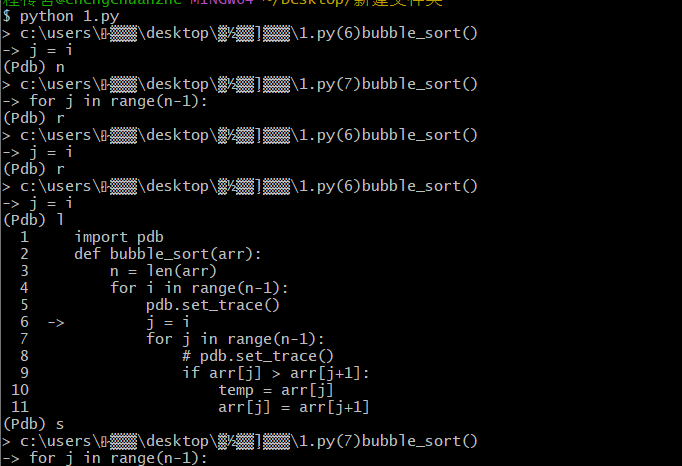
\includegraphics[scale=0.5]{1.png}
        \caption{pdb调试器}
        \label{figure}
    \end{figure}
    \begin{tabular}{|r|l|}
        \hline
        -l   & 显示当前行附近的 11 行或继续执行之前的显示  \\
        \hline 
        -s   & 执行当前行,并在第一个可能的地方停止  \\
        \hline 
        -n   & 继续执行直到当前函数的下一条语句或者 return 语句  \\
        \hline 
        -b   & 设置断点(基于传入的参数)  \\
        \hline 
        -p   &  在当前上下文对表达式求值并打印结果  \\
        \hline 
        -r   & 继续执行直到当前函数返回  \\
        \hline 
        -q   & 退出调试器  \\
        \hline 
      \end{tabular}
  \item{\large 静态分析}
    \begin{itemize}
        \item 静态分析的优势在于不用执行程序便可以发现代码的问题所在
    \end{itemize}
    \begin{lstlisting}[language = python]
import time

def foo():
    return 42

for foo in range(5):
    print(foo)
bar = 1
bar *= 0.2
time.sleep(60)
print(baz) # baz is not bar ,it is wrong
    \end{lstlisting}
    \begin{figure}[htbp]
      \centering
      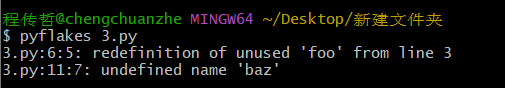
\includegraphics[scale=0.9]{2.png}
      \caption{静态分析}
      \label{figure}
    \end{figure} 
  \item{\large 计时}
    \\记录执行时间\\ \\
    \begin{lstlisting}[language = python]
import time, random
n = random.randint(1, 10) * 100

start = time.time()

print("Sleeping for {} ms".format(n))
time.sleep(n/1000)

print(time.time() - start)
    \end{lstlisting}
    运行结果
    \begin{lstlisting}
Sleeping for 800 ms
0.8006622791290283
    \end{lstlisting}
  \item{\large 性能分析工具}
  \\ 源代码
  \begin{lstlisting}[language = python]
import sys, re
def grep(pattern, file):
    with open(file, 'r') as f:
        print(file)
        for i, line in enumerate(f.readlines()):
            pattern = re.compile(pattern)
            match = pattern.search(line)
            if match is not None:
                print("{}: {}".format(i, line), end="")
if __name__ == '__main__':
    times = int(sys.argv[1])
    pattern = sys.argv[2]
    for i in range(times):
        for file in sys.argv[3:]:
            grep(pattern, file)
  \end{lstlisting}
  执行语句
  \begin{lstlisting}
$ python -m cProfile -s tottime grep.py 1000 '^(import|\s*def)[^,]*$' *.py
  \end{lstlisting}
  \item{\large 可视化}
    \begin{itemize}
        \item 使用述分析器的时候会输出大量信息,因此使用可视化输出结果能很好的帮助我们调试分析
    \end{itemize}
\end{enumerate}
\subsection{元编程}
\begin{enumerate}
  \item{\large makefile构建系统}
    \begin{itemize}
        \item 一个构建系统包括构建目标,相关依赖和规则都需要在makefile中定义
    \end{itemize}
    例如:
    \begin{lstlisting}
paper.pdf: paper.tex plot-data.png
	pdflatex paper.tex
plot-%.png: %.dat plot.py
	./plot.py -i $*.dat -o $@
    \end{lstlisting}
  \item{\large make使用}
    \\简单示例:
    \begin{lstlisting}[language = python]
print("hello world")
    \end{lstlisting}
    上面写入一个a.py的文件 \\
    makefile:
    \begin{lstlisting}
1_make:a.py
    python a.py -i
    \end{lstlisting}
    执行:
    \begin{lstlisting}
make
    \end{lstlisting}    
    输出结果
    \begin{figure}[htbp]
      \centering
      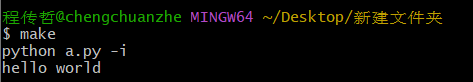
\includegraphics[scale=1]{3.png}
      \caption{make}
      \label{figure}
    \end{figure}
  \item{\large 依赖来源}
    \begin{itemize}
        \item 项目的依赖可能是本身也可能是其他项目,现在大多数的依赖可以通过某些软件仓库来获取
    \end{itemize}
  \item{\large 依赖API}
    \begin{itemize}
        \item 项目的依赖的项目在每次发布的时候都会创建一个版本号,类似python3.5,python3.7,他的格式是主版本号
            .次版本号.补丁号
        \item 版本号相关规则:
            \begin{itemize}
                \item 如果新的版本没有改变 API,请将补丁号递增
                \item 如果您添加了 API 并且该改动是向后兼容的,请将次版本号递增
                \item 如果您修改了 API 但是它并不向后兼容,请将主版本号递增
            \end{itemize}
    \end{itemize}
\end{enumerate}
\subsection{大杂烩}
\begin{enumerate}
  \item{\large Markdown}
    \begin{itemize}
        \item Markdown是一个轻量化的标记语言
    \end{itemize}
    Markdown的使用方式较为简单:\\
    \\
    \begin{figure}
      \centering
      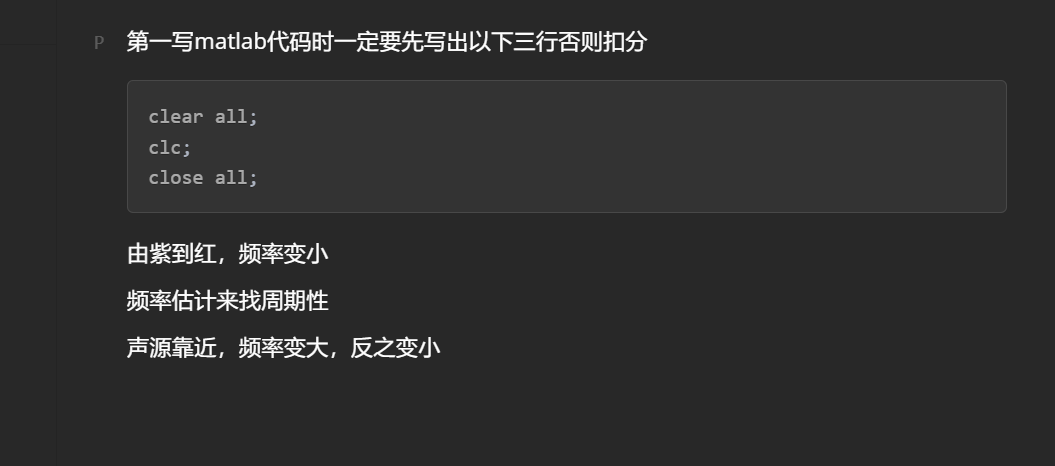
\includegraphics[scale = 0.5]{4.png}
      \caption{Markdown}
      \label{figure}
    \end{figure}
  \item{\large 修改键位映射}
    \begin{itemize}
        \item 推荐修改键位是因为键盘上很多不常用的功能却占用了比较方便的按键位置,例如CapsLock
        \item 推荐Windows在控制面板中修改
    \end{itemize}
  \item{\large API}
    \begin{itemize}
        \item API 通俗易懂的来讲就是封装操作,应用程序编程接口
    \end{itemize}
  \item{\large VPN}
    \begin{itemize}
        \item 发出的流量看上去来源于 VPN 供应商的网络而不是你的“真实”地址,而你实际接入的网络只能看到加密的流量
    \end{itemize}
\end{enumerate}
\subsection{Pytorch}
\begin{enumerate}
  \item{\large tensor初始化}
    \begin{itemize}
        \item 不同方式初始化tensor
    \end{itemize}
    \begin{lstlisting}[language = python]
import torch
import numpy as np

data = [[1, 2],[3, 4]]
x_data = torch.tensor(data)

np_array = np.array(data)
x_np = torch.from_numpy(np_array)

x_ones = torch.ones_like(x_data)
print(f"Ones Tensor: \n {x_ones} \n")

x_rand = torch.rand_like(x_data, dtype=torch.float) 
print(f"Random Tensor: \n {x_rand} \n")

shape = (2,3,)
rand_tensor = torch.rand(shape)
ones_tensor = torch.ones(shape)
zeros_tensor = torch.zeros(shape)

print(f"Random Tensor: \n {rand_tensor} \n")
print(f"Ones Tensor: \n {ones_tensor} \n")
print(f"Zeros Tensor: \n {zeros_tensor}")
    \end{lstlisting}[language = python]
  \item{\large tensor属性}
    \begin{lstlisting}
tensor = torch.rand(3,4)

print(f"Shape of tensor: {tensor.shape}")
print(f"Datatype of tensor: {tensor.dtype}")
print(f"Device tensor is stored on: {tensor.device}")
    \end{lstlisting}
    \begin{itemize}
        \item 三行四列
        \item float32浮点数
        \item CPU
    \end{itemize}
    tensor 剩下的操作很多使用的情况类似numpy的array数组,算数,线代,矩阵算式等等\\
  \item{\large 加载可视化数据集}
    \begin{lstlisting}[language = python]
import torch
from torch.utils.data import Dataset
from torchvision import datasets
from torchvision.transforms import ToTensor
import matplotlib.pyplot as plt


training_data = datasets.FashionMNIST(
    root="data",
    train=True,
    download=True,
    transform=ToTensor()
)

test_data = datasets.FashionMNIST(
    root="data",
    train=False,
    download=True,
    transform=ToTensor()
)

labels_map = {
    0: "T-Shirt",
    1: "Trouser",
    2: "Pullover",
    3: "Dress",
    4: "Coat",
    5: "Sandal",
    6: "Shirt",
    7: "Sneaker",
    8: "Bag",
    9: "Ankle Boot",
}
figure = plt.figure(figsize=(8, 8))
cols, rows = 3, 3
for i in range(1, cols * rows + 1):
    sample_idx = torch.randint(len(training_data), size=(1,)).item()
    img, label = training_data[sample_idx]
    figure.add_subplot(rows, cols, i)
    plt.title(labels_map[label])
    plt.axis("off")
    plt.imshow(img.squeeze(), cmap="gray")
plt.show()
    \end{lstlisting}
    
    \begin{figure}
      \centering
      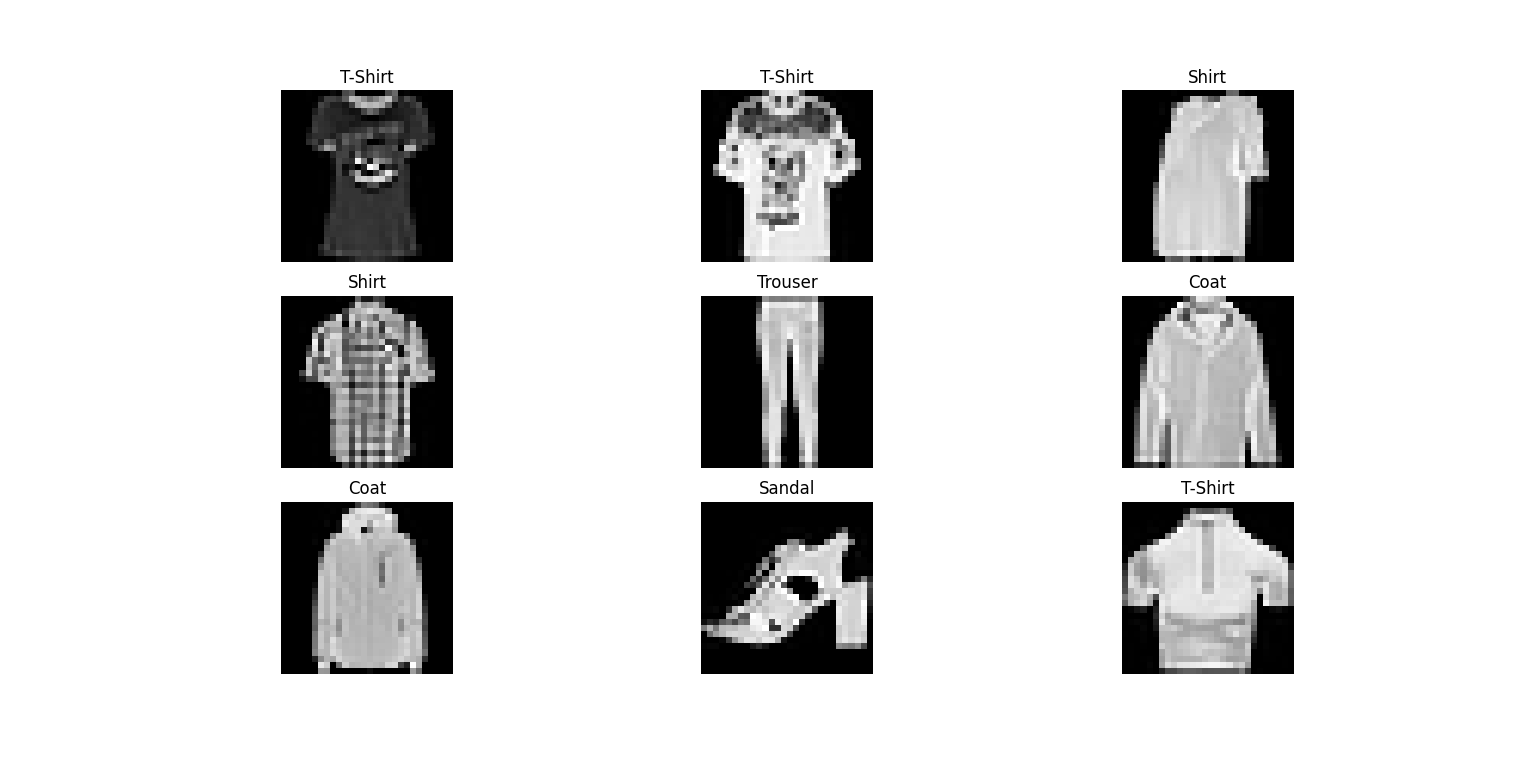
\includegraphics[scale=0.4]{5.png}
      \caption{数据集}
      \label{figure}
    \end{figure}
  \item{\large 转换}
    数据并不总是以所需的最终处理形式出现,需要转换
    \begin{lstlisting}[language = python]
import torch
from torchvision import datasets
from torchvision.transforms import ToTensor, Lambda

ds = datasets.FashionMNIST(
    root="data",
    train=True,
    download=True,
    transform=ToTensor(),
    target_transform=Lambda(lambda y: torch.zeros(10, dtype=torch.float).scatter_(0, torch.tensor(y), value=1))
)
    \end{lstlisting}
  \item{\large 自定义运算符}
    \begin{itemize}
        \item 必须通过 Python torch.library 文档或 C++ API 向 PyTorch 注册自定义操作
    \end{itemize}
\end{enumerate}
\section{Github链接}
https://github.com/Chengchuanzhe/-.git
\section{学习感悟}
    元编程是编程的编程,它允许我们在更高层次上操作代码本身,如修改代码结构、生成代码等。学习元编程让我深刻体会到编程的灵活性和抽象能力的极限。Python中的装饰器、元类以及反射机制是元编程的强有力工具。掌握这些工具后,我发现自己能够更优雅地解决一些复杂的设计问题,比如动态生成类、运行时修改函数行为等。元编程是进阶编程技能的关键一环,值得深入探索。Markdown以其简洁的语法和强大的功能,迅速成为了我写作和记录的首选工具。它不仅易于学习,而且能够高效地生成结构清晰、格式美观的文档。从笔记整理到项目报告,Markdown都能轻松应对。最让我喜欢的是Markdown与Git、GitHub等版本控制系统的完美结合,使得文档的编写、分享和协作变得更加便捷。调试是编程过程中不可或缺的一环,它教会了我如何系统地定位和解决问题。从最初的盲目试错,到后来的使用调试工具(如Python的pdb)、打印日志、分段执行等策略,我的调试技能有了显著提升。更重要的是,我学会了如何设计易于调试的代码,比如遵循良好的命名规范、编写清晰的注释、使用断言来验证假设等。PyTorch作为一款流行的深度学习框架,以其灵活性和易用性著称。学习PyTorch让我深入理解了深度学习的基本原理,并亲手实践了多个经典模型,如卷积神经网络(CNN)、循环神经网络(RNN)等。PyTorch的动态图特性使得模型的开发和调试变得异常简单,极大地提高了我的开发效率。同时,PyTorch丰富的社区资源也让我在遇到问题时能够快速找到解决方案。
\end{document} 